\documentclass[12pt,b5paper]{ltjsarticle}

%\usepackage[margin=15truemm, top=5truemm, bottom=5truemm]{geometry}
\usepackage[margin=15truemm]{geometry}

\usepackage{amsmath,amssymb}
%\pagestyle{headings}
\pagestyle{empty}

%\usepackage{listings,url}
\renewcommand{\theenumi}{(\arabic{enumi})}

\usepackage{graphicx}

\usepackage{tikz}
\usetikzlibrary {arrows.meta}
\usepackage{wrapfig}	% required for `\wrapfigure' (yatex added)

%% 像Im を定義
%\newcommand{\Img}{\mathop{\mathrm{Im}}\nolimits}

\begin{document}

\textbf{$\varepsilon$ - $\delta$ (イプシロン - デルタ) 論法}

関数の極限を定義する為の論法である。
単純に極限
$\displaystyle \left( \lim_{x \rightarrow \alpha}f(x)=f(\alpha) \right)$
を
定義する場合のほか、
関数の連続性を定義する場合にも利用する。

\hrulefill \:
 \textbf{定義 関数の連続}
\: \hrulefill

%区間$I\subset $
\fbox{
$\mathbb{R}$上で定義された関数$f(x)$が点$a\in\mathbb{R}$で連続である
}

$\stackrel{\mathrm{def}}{\Leftrightarrow}$
\quad 任意の正の実数$\varepsilon$に対し、次の条件を満たす正の実数$\delta$が存在する
\begin{center}
 [\textbf{条件}]\quad
 %区間$I$の任意の点$x$に対し
 $\lvert x-a \rvert < \delta$ であるなら
 $\lvert f(x)-f(a) \rvert < \varepsilon$ である。
\end{center}

\dotfill

記号で書くと次の通り
\begin{equation}
 {}^\forall \varepsilon >0 , \; {}^\exists \delta > 0 \quad
  s.t. \quad
  %{}^\forall x \in I ,  \;
  \lvert x-a \rvert  < \delta \Rightarrow \lvert f(x)-f(a) \rvert < \varepsilon
  \tag{\spadesuit}
\end{equation}


\hrulefill

\begin{wrapfigure}[8]{r}{200pt}
 \vspace*{-40pt}
 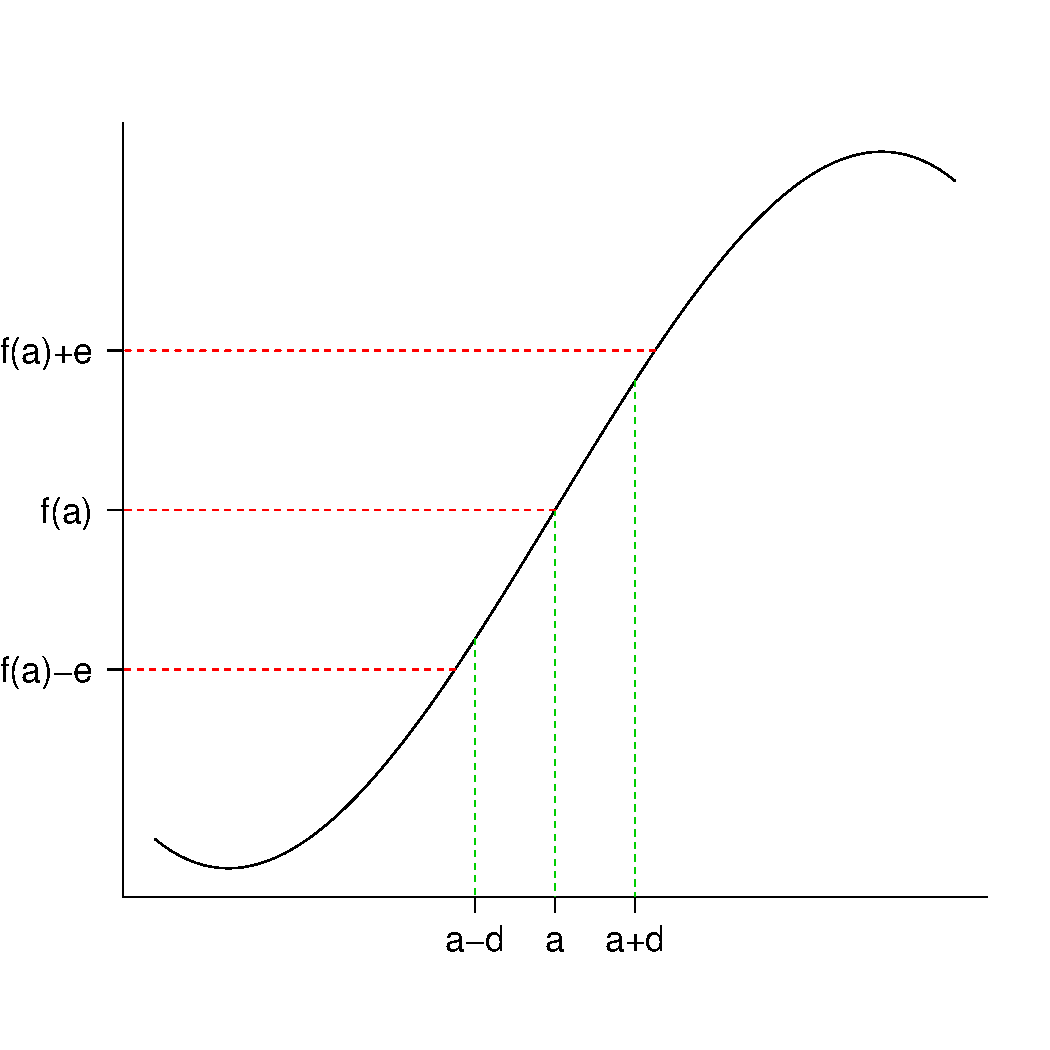
\includegraphics[width=200pt]{eps_del.pdf}
\end{wrapfigure}

\textbf{[解説]}

%$\varepsilon - \delta$論法では
関数の連続を考える場合、
記号等は次のような順に決定する。
\begin{enumerate}
 \item 関数$f(x)$
 \item 点$a \in \mathbb{R}$
       \label{155728_3May22}
 \item 実数$\varepsilon >0$
 \item 実数$\delta >0$
       \label{203617_29Apr22}
\end{enumerate}
%前半の2つ($f(x), a\in\mathbb{R}$)は連続性を示すべき条件として、
%後半の2つ($\varepsilon >0, \; \delta >0$)は連続性を示す証明の中で決定。

\ref{203617_29Apr22}
の$\delta$
は条件
「$\lvert x-a \rvert  < \delta \Rightarrow \lvert f(x)-f(a) \rvert < \varepsilon$」
を満たすものが一つ存在すればよく、
右上のグラフのような位置関係を意味している。
{\footnotesize (グラフの記号は$\varepsilon$の代わりに e 、$\delta$の代わりに d を利用)}

$\varepsilon$がどんな値であっても、
$\varepsilon$に対して
$\delta$が存在することが
連続の定義となる。
%
%が存在することを確認する。
%この$\delta$がどんな$\varepsilon$であっても必ず存在することで
%「1点$a\in\mathbb{R}$にて$f(x)$が連続」を定義する。
%
集合で書けば、次のような式を満たす$\delta$があることを定義としている。
\begin{equation}
 (f(a-\delta), f(a+\delta)) \subset (f(a)-\varepsilon, f(a)+\varepsilon)
  \tag{\heartsuit}\label{154609_3May22}
\end{equation}

$\varepsilon$は任意の値なので大きくても小さくてもいいが、
大きい場合は$\delta$も存在を見つけやすいので、
$\varepsilon$がとても小さい場合を調べることが重要である。

もし不連続であれば、
$\varepsilon$が十分に小さいと
$(f(a)-\varepsilon, f(a)+\varepsilon)$の端に
グラフがない事が起きる。
この場合、$\delta$はどんな値を取っても
式(\ref{154609_3May22})を満たすことが出来ない。



%\begin{equation}
% {}^\forall \varepsilon >0 , \; {}^\exists \delta > 0 \quad
%  s.t. \quad
%  \lvert x-a \rvert  < \delta \Rightarrow \lvert f(x)-f(a) \rvert < \varepsilon
%\end{equation}


%$\varepsilon$を一つ決定する。
%区間$(f(a)-\varepsilon , f(a)+\varepsilon)$
%に対し

記号の決定の\ref{155728_3May22} $a\in\mathbb{R}$ がある区間上の任意の点だとすれば区間上で連続という。

\end{document}
